\documentclass[1p]{elsarticle_modified}
%\bibliographystyle{elsarticle-num}

%\usepackage[colorlinks]{hyperref}
%\usepackage{abbrmath_seonhwa} %\Abb, \Ascr, \Acal ,\Abf, \Afrak
\usepackage{amsfonts}
\usepackage{amssymb}
\usepackage{amsmath}
\usepackage{amsthm}
\usepackage{scalefnt}
\usepackage{amsbsy}
\usepackage{kotex}
\usepackage{caption}
\usepackage{subfig}
\usepackage{color}
\usepackage{graphicx}
\usepackage{xcolor} %% white, black, red, green, blue, cyan, magenta, yellow
\usepackage{float}
\usepackage{setspace}
\usepackage{hyperref}

\usepackage{tikz}
\usetikzlibrary{arrows}

\usepackage{multirow}
\usepackage{array} % fixed length table
\usepackage{hhline}

%%%%%%%%%%%%%%%%%%%%%
\makeatletter
\renewcommand*\env@matrix[1][\arraystretch]{%
	\edef\arraystretch{#1}%
	\hskip -\arraycolsep
	\let\@ifnextchar\new@ifnextchar
	\array{*\c@MaxMatrixCols c}}
\makeatother %https://tex.stackexchange.com/questions/14071/how-can-i-increase-the-line-spacing-in-a-matrix
%%%%%%%%%%%%%%%

\usepackage[normalem]{ulem}

\newcommand{\msout}[1]{\ifmmode\text{\sout{\ensuremath{#1}}}\else\sout{#1}\fi}
%SOURCE: \msout is \stkout macro in https://tex.stackexchange.com/questions/20609/strikeout-in-math-mode

\newcommand{\cancel}[1]{
	\ifmmode
	{\color{red}\msout{#1}}
	\else
	{\color{red}\sout{#1}}
	\fi
}

\newcommand{\add}[1]{
	{\color{blue}\uwave{#1}}
}

\newcommand{\replace}[2]{
	\ifmmode
	{\color{red}\msout{#1}}{\color{blue}\uwave{#2}}
	\else
	{\color{red}\sout{#1}}{\color{blue}\uwave{#2}}
	\fi
}

\newcommand{\Sol}{\mathcal{S}} %segment
\newcommand{\D}{D} %diagram
\newcommand{\A}{\mathcal{A}} %arc


%%%%%%%%%%%%%%%%%%%%%%%%%%%%%5 test

\def\sl{\operatorname{\textup{SL}}(2,\Cbb)}
\def\psl{\operatorname{\textup{PSL}}(2,\Cbb)}
\def\quan{\mkern 1mu \triangleright \mkern 1mu}

\theoremstyle{definition}
\newtheorem{thm}{Theorem}[section]
\newtheorem{prop}[thm]{Proposition}
\newtheorem{lem}[thm]{Lemma}
\newtheorem{ques}[thm]{Question}
\newtheorem{cor}[thm]{Corollary}
\newtheorem{defn}[thm]{Definition}
\newtheorem{exam}[thm]{Example}
\newtheorem{rmk}[thm]{Remark}
\newtheorem{alg}[thm]{Algorithm}

\newcommand{\I}{\sqrt{-1}}
\begin{document}

%\begin{frontmatter}
%
%\title{Boundary parabolic representations of knots up to 8 crossings}
%
%%% Group authors per affiliation:
%\author{Yunhi Cho} 
%\address{Department of Mathematics, University of Seoul, Seoul, Korea}
%\ead{yhcho@uos.ac.kr}
%
%
%\author{Seonhwa Kim} %\fnref{s_kim}}
%\address{Center for Geometry and Physics, Institute for Basic Science, Pohang, 37673, Korea}
%\ead{ryeona17@ibs.re.kr}
%
%\author{Hyuk Kim}
%\address{Department of Mathematical Sciences, Seoul National University, Seoul 08826, Korea}
%\ead{hyukkim@snu.ac.kr}
%
%\author{Seokbeom Yoon}
%\address{Department of Mathematical Sciences, Seoul National University, Seoul, 08826,  Korea}
%\ead{sbyoon15@snu.ac.kr}
%
%\begin{abstract}
%We find all boundary parabolic representation of knots up to 8 crossings.
%
%\end{abstract}
%\begin{keyword}
%    \MSC[2010] 57M25 
%\end{keyword}
%
%\end{frontmatter}

%\linenumbers
%\tableofcontents
%
\newcommand\colored[1]{\textcolor{white}{\rule[-0.35ex]{0.8em}{1.4ex}}\kern-0.8em\color{red} #1}%
%\newcommand\colored[1]{\textcolor{white}{ #1}\kern-2.17ex	\textcolor{white}{ #1}\kern-1.81ex	\textcolor{white}{ #1}\kern-2.15ex\color{red}#1	}

{\Large $\underline{10_{108}~(K10a_{119})}$}

\setlength{\tabcolsep}{10pt}
\renewcommand{\arraystretch}{1.6}
\vspace{1cm}\begin{tabular}{m{100pt}>{\centering\arraybackslash}m{274pt}}
\multirow{5}{120pt}{
	\centering
	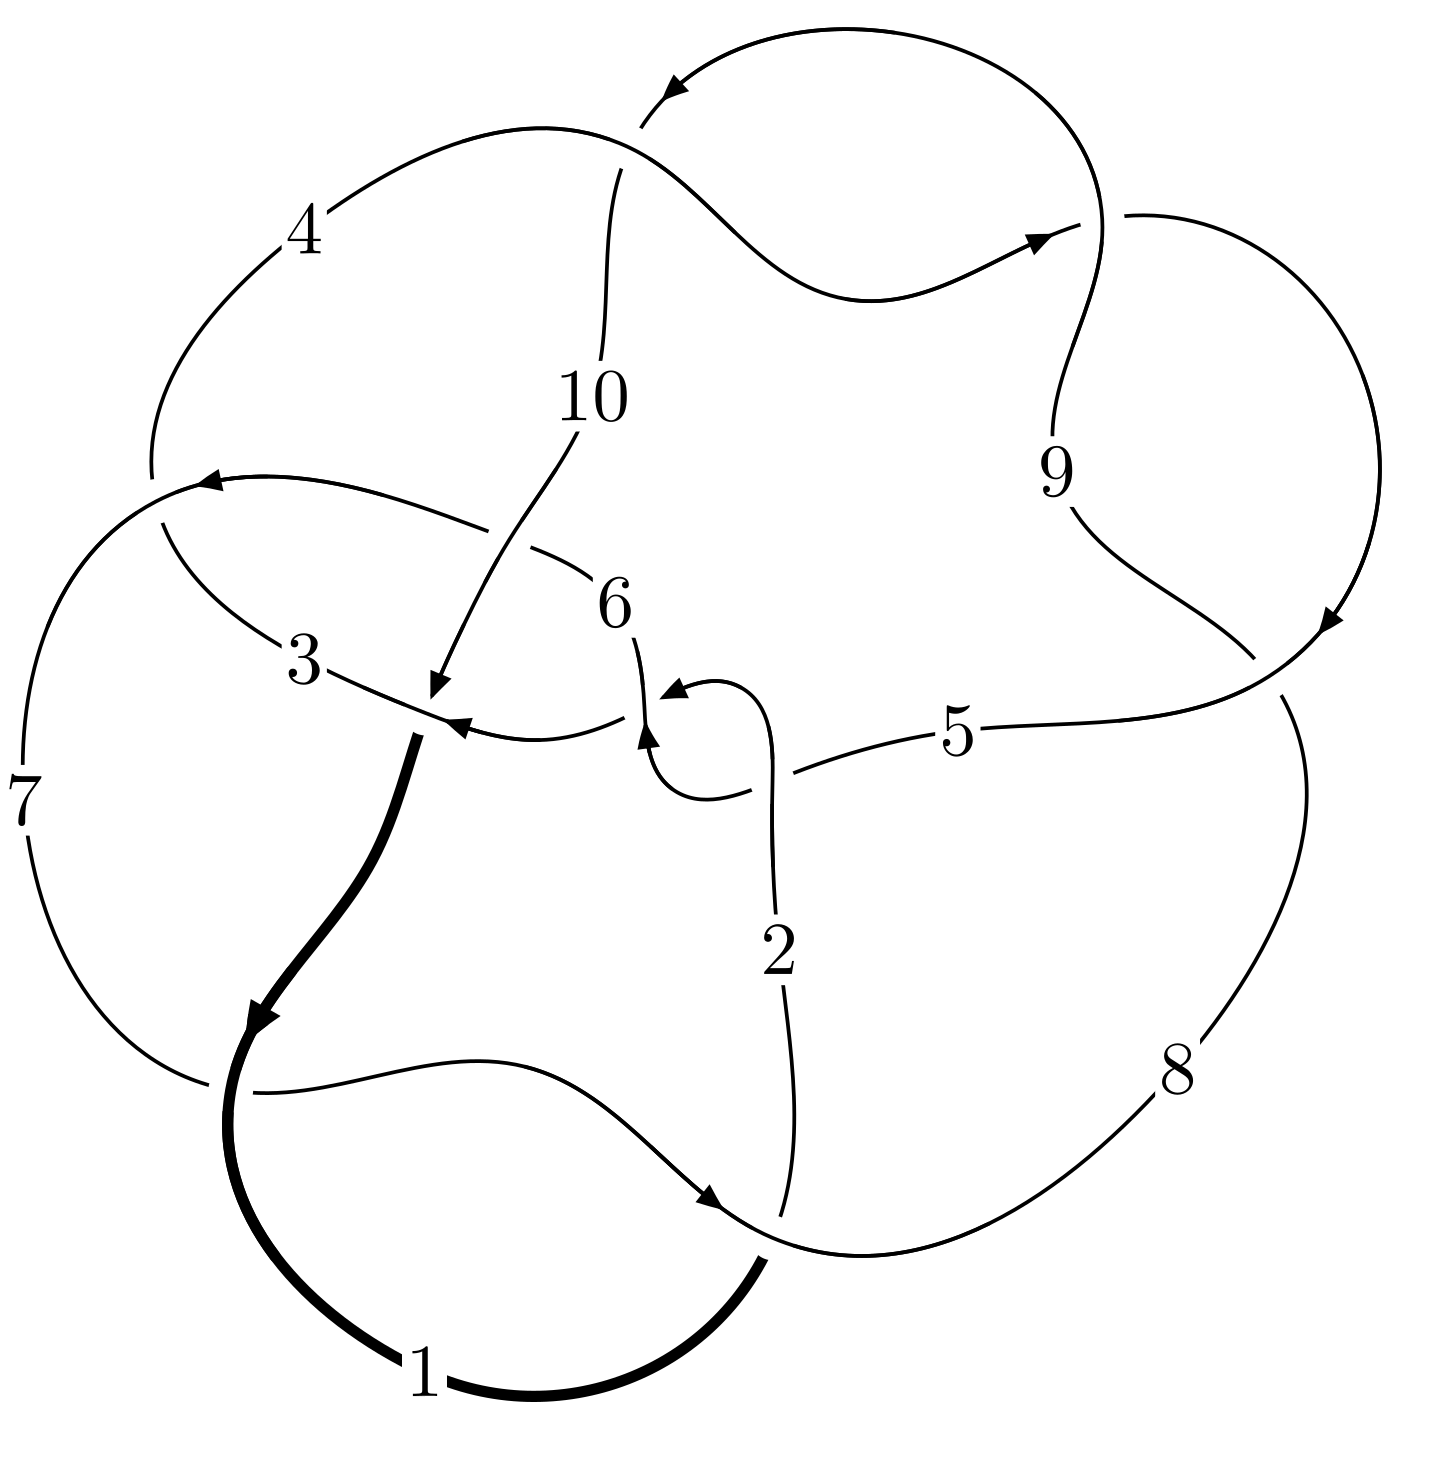
\includegraphics[width=112pt]{../../../GIT/diagram.site/Diagrams/png/192_10_108.png}\\
\ \ \ A knot diagram\footnotemark}&
\allowdisplaybreaks
\textbf{Linearized knot diagam} \\
\cline{2-2}
 &
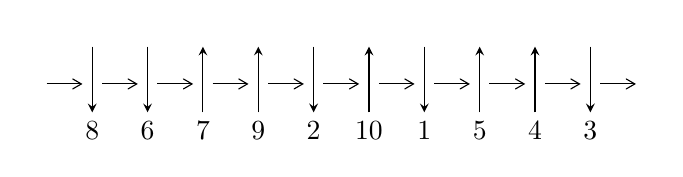
\begin{tikzpicture}[x=20pt, y=17pt]
	% nodes
	\node (C0) at (0, 0) {};
	\node (C1) at (1, 0) {};
	\node (C1U) at (1, +1) {};
	\node (C1D) at (1, -1) {8};

	\node (C2) at (2, 0) {};
	\node (C2U) at (2, +1) {};
	\node (C2D) at (2, -1) {6};

	\node (C3) at (3, 0) {};
	\node (C3U) at (3, +1) {};
	\node (C3D) at (3, -1) {7};

	\node (C4) at (4, 0) {};
	\node (C4U) at (4, +1) {};
	\node (C4D) at (4, -1) {9};

	\node (C5) at (5, 0) {};
	\node (C5U) at (5, +1) {};
	\node (C5D) at (5, -1) {2};

	\node (C6) at (6, 0) {};
	\node (C6U) at (6, +1) {};
	\node (C6D) at (6, -1) {10};

	\node (C7) at (7, 0) {};
	\node (C7U) at (7, +1) {};
	\node (C7D) at (7, -1) {1};

	\node (C8) at (8, 0) {};
	\node (C8U) at (8, +1) {};
	\node (C8D) at (8, -1) {5};

	\node (C9) at (9, 0) {};
	\node (C9U) at (9, +1) {};
	\node (C9D) at (9, -1) {4};

	\node (C10) at (10, 0) {};
	\node (C10U) at (10, +1) {};
	\node (C10D) at (10, -1) {3};
	\node (C11) at (11, 0) {};

	% arrows
	\draw[->,>={angle 60}]
	(C0) edge (C1) (C1) edge (C2) (C2) edge (C3) (C3) edge (C4) (C4) edge (C5) (C5) edge (C6) (C6) edge (C7) (C7) edge (C8) (C8) edge (C9) (C9) edge (C10) (C10) edge (C11) ;	\draw[->,>=stealth]
	(C1U) edge (C1D) (C2U) edge (C2D) (C3D) edge (C3U) (C4D) edge (C4U) (C5U) edge (C5D) (C6D) edge (C6U) (C7U) edge (C7D) (C8D) edge (C8U) (C9D) edge (C9U) (C10U) edge (C10D) ;
	\end{tikzpicture} \\
\hhline{~~} \\& 
\textbf{Solving Sequence} \\ \cline{2-2} 
 &
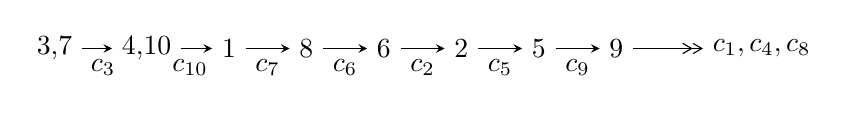
\begin{tikzpicture}[x=28pt, y=7pt]
	% node
	\node (A0) at (-1/8, 0) {3,7};
	\node (A1) at (17/16, 0) {4,10};
	\node (A2) at (17/8, 0) {1};
	\node (A3) at (25/8, 0) {8};
	\node (A4) at (33/8, 0) {6};
	\node (A5) at (41/8, 0) {2};
	\node (A6) at (49/8, 0) {5};
	\node (A7) at (57/8, 0) {9};
	\node (C1) at (1/2, -1) {$c_{3}$};
	\node (C2) at (13/8, -1) {$c_{10}$};
	\node (C3) at (21/8, -1) {$c_{7}$};
	\node (C4) at (29/8, -1) {$c_{6}$};
	\node (C5) at (37/8, -1) {$c_{2}$};
	\node (C6) at (45/8, -1) {$c_{5}$};
	\node (C7) at (53/8, -1) {$c_{9}$};
	\node (A8) at (9, 0) {$c_{1},c_{4},c_{8}$};

	% edge
	\draw[->,>=stealth]	
	(A0) edge (A1) (A1) edge (A2) (A2) edge (A3) (A3) edge (A4) (A4) edge (A5) (A5) edge (A6) (A6) edge (A7) ;
	\draw[->>,>={angle 60}]	
	(A7) edge (A8);
\end{tikzpicture} \\ 

\end{tabular} \\

\footnotetext{
The image of knot diagram is generated by the software ``\textbf{Draw programme}" developed by Andrew Bartholomew(\url{http://www.layer8.co.uk/maths/draw/index.htm\#Running-draw}), where we modified some parts for our purpose(\url{https://github.com/CATsTAILs/LinksPainter}).
}\phantom \\ \newline 
\centering \textbf{Ideals for irreducible components\footnotemark of $X_{\text{par}}$} 
 
\begin{align*}
I^u_{1}&=\langle 
-11 u^{13}-5 u^{12}+\cdots+4 b+21,\;a-1,\\
\phantom{I^u_{1}}&\phantom{= \langle  }u^{14}+3 u^{12}- u^{11}+10 u^{10}-2 u^9+12 u^8-2 u^7+12 u^6- u^5+5 u^4-4 u^3-2 u+1\rangle \\
I^u_{2}&=\langle 
-1.14931\times10^{20} u^{23}+8.36148\times10^{19} u^{22}+\cdots+1.67024\times10^{21} b+1.69140\times10^{22},\\
\phantom{I^u_{2}}&\phantom{= \langle  }-7.94884\times10^{24} u^{23}+4.40832\times10^{25} u^{22}+\cdots+8.43824\times10^{25} a+2.32671\times10^{27},\\
\phantom{I^u_{2}}&\phantom{= \langle  }u^{24}+3 u^{23}+\cdots+6 u+19\rangle \\
I^u_{3}&=\langle 
- u^6- u^5-3 u^3-3 u^2+2 b- u+1,\;a+1,\;u^7+u^5+u^4+2 u^3-1\rangle \\
\\
\end{align*}
\raggedright * 3 irreducible components of $\dim_{\mathbb{C}}=0$, with total 45 representations.\\
\footnotetext{All coefficients of polynomials are rational numbers. But the coefficients are sometimes approximated in decimal forms when there is not enough margin.}
\newpage
\renewcommand{\arraystretch}{1}
\centering \section*{I. $I^u_{1}= \langle -11 u^{13}-5 u^{12}+\cdots+4 b+21,\;a-1,\;u^{14}+3 u^{12}+\cdots-2 u+1 \rangle$}
\flushleft \textbf{(i) Arc colorings}\\
\begin{tabular}{m{7pt} m{180pt} m{7pt} m{180pt} }
\flushright $a_{3}=$&$\begin{pmatrix}1\\0\end{pmatrix}$ \\
\flushright $a_{7}=$&$\begin{pmatrix}0\\u\end{pmatrix}$ \\
\flushright $a_{4}=$&$\begin{pmatrix}1\\- u^2\end{pmatrix}$ \\
\flushright $a_{10}=$&$\begin{pmatrix}1\\\frac{11}{4} u^{13}+\frac{5}{4} u^{12}+\cdots-\frac{1}{4} u-\frac{21}{4}\end{pmatrix}$ \\
\flushright $a_{1}=$&$\begin{pmatrix}-\frac{11}{4} u^{13}-\frac{5}{4} u^{12}+\cdots+\frac{1}{4} u+\frac{25}{4}\\\frac{11}{4} u^{13}+\frac{5}{4} u^{12}+\cdots-\frac{1}{4} u-\frac{21}{4}\end{pmatrix}$ \\
\flushright $a_{8}=$&$\begin{pmatrix}\frac{7}{2} u^{13}+u^{12}+\cdots+\frac{1}{2} u-6\\-\frac{9}{4} u^{13}-\frac{1}{4} u^{12}+\cdots-\frac{1}{4} u+\frac{13}{4}\end{pmatrix}$ \\
\flushright $a_{6}=$&$\begin{pmatrix}- u\\-\frac{5}{4} u^{13}-\frac{3}{4} u^{12}+\cdots+\frac{3}{4} u+\frac{11}{4}\end{pmatrix}$ \\
\flushright $a_{2}=$&$\begin{pmatrix}-\frac{3}{4} u^{13}-\frac{1}{4} u^{12}+\cdots+\frac{1}{4} u+\frac{9}{4}\\u^{13}+\frac{1}{2} u^{12}+\cdots+u-\frac{7}{2}\end{pmatrix}$ \\
\flushright $a_{5}=$&$\begin{pmatrix}-\frac{7}{4} u^{13}-\frac{7}{4} u^{12}+\cdots+\frac{5}{4} u+\frac{15}{4}\\-\frac{1}{4} u^{13}+\frac{1}{4} u^{12}+\cdots+\frac{3}{4} u+\frac{3}{4}\end{pmatrix}$ \\
\flushright $a_{9}=$&$\begin{pmatrix}-\frac{11}{4} u^{13}-\frac{5}{4} u^{12}+\cdots+\frac{1}{4} u+\frac{25}{4}\\\frac{7}{2} u^{13}+\frac{3}{2} u^{12}+\cdots-\frac{1}{2} u-\frac{13}{2}\end{pmatrix}$\\&\end{tabular}
\flushleft \textbf{(ii) Obstruction class $= -1$}\\~\\
\flushleft \textbf{(iii) Cusp Shapes $= -\frac{63}{4} u^{13}-\frac{39}{4} u^{12}-49 u^{11}-\frac{61}{4} u^{10}-\frac{623}{4} u^9-\frac{289}{4} u^8-\frac{781}{4} u^7-\frac{407}{4} u^6-\frac{843}{4} u^5-125 u^4-\frac{479}{4} u^3-\frac{23}{4} u^2+\frac{41}{4} u+\frac{111}{4}$}\\~\\
\newpage\renewcommand{\arraystretch}{1}
\flushleft \textbf{(iv) u-Polynomials at the component}\newline \\
\begin{tabular}{m{50pt}|m{274pt}}
Crossings & \hspace{64pt}u-Polynomials at each crossing \\
\hline $$\begin{aligned}c_{1},c_{2},c_{5}\\c_{7}\end{aligned}$$&$\begin{aligned}
&u^{14}+u^{13}+\cdots+u+1
\end{aligned}$\\
\hline $$\begin{aligned}c_{3},c_{6}\end{aligned}$$&$\begin{aligned}
&u^{14}+3 u^{12}+\cdots+2 u+1
\end{aligned}$\\
\hline $$\begin{aligned}c_{4},c_{8},c_{9}\end{aligned}$$&$\begin{aligned}
&u^{14}-7 u^{13}+\cdots-56 u+8
\end{aligned}$\\
\hline $$\begin{aligned}c_{10}\end{aligned}$$&$\begin{aligned}
&u^{14}-13 u^{13}+\cdots-128 u+16
\end{aligned}$\\
\hline
\end{tabular}\\~\\
\newpage\renewcommand{\arraystretch}{1}
\flushleft \textbf{(v) Riley Polynomials at the component}\newline \\
\begin{tabular}{m{50pt}|m{274pt}}
Crossings & \hspace{64pt}Riley Polynomials at each crossing \\
\hline $$\begin{aligned}c_{1},c_{2},c_{5}\\c_{7}\end{aligned}$$&$\begin{aligned}
&y^{14}-15 y^{13}+\cdots+7 y+1
\end{aligned}$\\
\hline $$\begin{aligned}c_{3},c_{6}\end{aligned}$$&$\begin{aligned}
&y^{14}+6 y^{13}+\cdots-4 y+1
\end{aligned}$\\
\hline $$\begin{aligned}c_{4},c_{8},c_{9}\end{aligned}$$&$\begin{aligned}
&y^{14}+13 y^{13}+\cdots-32 y+64
\end{aligned}$\\
\hline $$\begin{aligned}c_{10}\end{aligned}$$&$\begin{aligned}
&y^{14}-3 y^{13}+\cdots-128 y+256
\end{aligned}$\\
\hline
\end{tabular}\\~\\
\newpage\flushleft \textbf{(vi) Complex Volumes and Cusp Shapes}
$$\begin{array}{c|c|c}  
\text{Solutions to }I^u_{1}& \I (\text{vol} + \sqrt{-1}CS) & \text{Cusp shape}\\
 \hline 
\begin{aligned}
u &= -0.449224 + 0.834596 I \\
a &= \phantom{-}1.00000\phantom{ +0.000000I} \\
b &= \phantom{-}1.63158 + 1.27198 I\end{aligned}
 & -6.03431 - 1.96052 I & -7.98588 + 3.63018 I \\ \hline\begin{aligned}
u &= -0.449224 - 0.834596 I \\
a &= \phantom{-}1.00000\phantom{ +0.000000I} \\
b &= \phantom{-}1.63158 - 1.27198 I\end{aligned}
 & -6.03431 + 1.96052 I & -7.98588 - 3.63018 I \\ \hline\begin{aligned}
u &= -0.078710 + 0.897903 I \\
a &= \phantom{-}1.00000\phantom{ +0.000000I} \\
b &= \phantom{-}1.17059 - 1.56821 I\end{aligned}
 & -13.45690 - 3.91206 I & -10.44278 + 2.90737 I \\ \hline\begin{aligned}
u &= -0.078710 - 0.897903 I \\
a &= \phantom{-}1.00000\phantom{ +0.000000I} \\
b &= \phantom{-}1.17059 + 1.56821 I\end{aligned}
 & -13.45690 + 3.91206 I & -10.44278 - 2.90737 I \\ \hline\begin{aligned}
u &= -0.605476 + 0.511603 I \\
a &= \phantom{-}1.00000\phantom{ +0.000000I} \\
b &= \phantom{-}0.410349 + 0.397635 I\end{aligned}
 & \phantom{-}1.004190 - 0.960325 I & \phantom{-}4.75919 + 2.76007 I \\ \hline\begin{aligned}
u &= -0.605476 - 0.511603 I \\
a &= \phantom{-}1.00000\phantom{ +0.000000I} \\
b &= \phantom{-}0.410349 - 0.397635 I\end{aligned}
 & \phantom{-}1.004190 + 0.960325 I & \phantom{-}4.75919 - 2.76007 I \\ \hline\begin{aligned}
u &= \phantom{-}0.777537 + 1.051940 I \\
a &= \phantom{-}1.00000\phantom{ +0.000000I} \\
b &= \phantom{-}0.686906 - 0.276246 I\end{aligned}
 & -4.00326 + 3.48344 I & \phantom{-}0.15043 - 1.66516 I \\ \hline\begin{aligned}
u &= \phantom{-}0.777537 - 1.051940 I \\
a &= \phantom{-}1.00000\phantom{ +0.000000I} \\
b &= \phantom{-}0.686906 + 0.276246 I\end{aligned}
 & -4.00326 - 3.48344 I & \phantom{-}0.15043 + 1.66516 I \\ \hline\begin{aligned}
u &= \phantom{-}0.803725 + 1.091800 I \\
a &= \phantom{-}1.00000\phantom{ +0.000000I} \\
b &= \phantom{-}1.43309 - 0.98357 I\end{aligned}
 & -6.98628 + 8.54350 I & -5.70825 - 6.73218 I \\ \hline\begin{aligned}
u &= \phantom{-}0.803725 - 1.091800 I \\
a &= \phantom{-}1.00000\phantom{ +0.000000I} \\
b &= \phantom{-}1.43309 + 0.98357 I\end{aligned}
 & -6.98628 - 8.54350 I & -5.70825 + 6.73218 I\\
 \hline 
 \end{array}$$\newpage$$\begin{array}{c|c|c}  
\text{Solutions to }I^u_{1}& \I (\text{vol} + \sqrt{-1}CS) & \text{Cusp shape}\\
 \hline 
\begin{aligned}
u &= \phantom{-}0.497537 + 0.019222 I \\
a &= \phantom{-}1.00000\phantom{ +0.000000I} \\
b &= -0.118230 + 0.827768 I\end{aligned}
 & -0.78382 + 1.56236 I & -0.68409 - 4.99180 I \\ \hline\begin{aligned}
u &= \phantom{-}0.497537 - 0.019222 I \\
a &= \phantom{-}1.00000\phantom{ +0.000000I} \\
b &= -0.118230 - 0.827768 I\end{aligned}
 & -0.78382 - 1.56236 I & -0.68409 + 4.99180 I \\ \hline\begin{aligned}
u &= -0.94539 + 1.37947 I \\
a &= \phantom{-}1.00000\phantom{ +0.000000I} \\
b &= \phantom{-}1.28571 + 0.96390 I\end{aligned}
 & -14.9753 - 12.9046 I & -7.08862 + 6.20783 I \\ \hline\begin{aligned}
u &= -0.94539 - 1.37947 I \\
a &= \phantom{-}1.00000\phantom{ +0.000000I} \\
b &= \phantom{-}1.28571 - 0.96390 I\end{aligned}
 & -14.9753 + 12.9046 I & -7.08862 - 6.20783 I\\
 \hline 
 \end{array}$$\newpage\newpage\renewcommand{\arraystretch}{1}
\centering \section*{II. $I^u_{2}= \langle -1.15\times10^{20} u^{23}+8.36\times10^{19} u^{22}+\cdots+1.67\times10^{21} b+1.69\times10^{22},\;-7.95\times10^{24} u^{23}+4.41\times10^{25} u^{22}+\cdots+8.44\times10^{25} a+2.33\times10^{27},\;u^{24}+3 u^{23}+\cdots+6 u+19 \rangle$}
\flushleft \textbf{(i) Arc colorings}\\
\begin{tabular}{m{7pt} m{180pt} m{7pt} m{180pt} }
\flushright $a_{3}=$&$\begin{pmatrix}1\\0\end{pmatrix}$ \\
\flushright $a_{7}=$&$\begin{pmatrix}0\\u\end{pmatrix}$ \\
\flushright $a_{4}=$&$\begin{pmatrix}1\\- u^2\end{pmatrix}$ \\
\flushright $a_{10}=$&$\begin{pmatrix}0.0942002 u^{23}-0.522421 u^{22}+\cdots-0.770681 u-27.5734\\0.0688111 u^{23}-0.0500614 u^{22}+\cdots-0.114391 u-10.1267\end{pmatrix}$ \\
\flushright $a_{1}=$&$\begin{pmatrix}0.0253891 u^{23}-0.472360 u^{22}+\cdots-0.656290 u-17.4468\\0.0688111 u^{23}-0.0500614 u^{22}+\cdots-0.114391 u-10.1267\end{pmatrix}$ \\
\flushright $a_{8}=$&$\begin{pmatrix}0.210439 u^{23}-0.295381 u^{22}+\cdots+0.388096 u-30.0893\\0.142257 u^{23}+0.385777 u^{22}+\cdots+6.96971 u+1.18135\end{pmatrix}$ \\
\flushright $a_{6}=$&$\begin{pmatrix}0.412085 u^{23}+0.307609 u^{22}+\cdots+8.81510 u-23.1359\\0.0593893 u^{23}+0.217213 u^{22}+\cdots+3.45729 u+5.77204\end{pmatrix}$ \\
\flushright $a_{2}=$&$\begin{pmatrix}-1.13112 u^{23}-2.14478 u^{22}+\cdots-38.0006 u+30.5997\\-0.121067 u^{23}-0.349984 u^{22}+\cdots-8.56109 u-3.83752\end{pmatrix}$ \\
\flushright $a_{5}=$&$\begin{pmatrix}-1.76389 u^{23}-5.24938 u^{22}+\cdots-57.7044 u-1.81964\\-0.503760 u^{23}-1.53601 u^{22}+\cdots-18.2795 u-3.57211\end{pmatrix}$ \\
\flushright $a_{9}=$&$\begin{pmatrix}-0.0384844 u^{23}-1.08724 u^{22}+\cdots-3.69662 u-32.7422\\-0.0389677 u^{23}-0.469297 u^{22}+\cdots-3.63598 u-13.2952\end{pmatrix}$\\&\end{tabular}
\flushleft \textbf{(ii) Obstruction class $= -1$}\\~\\
\flushleft \textbf{(iii) Cusp Shapes $= -\frac{6347129273848677988188136}{4441180884722885954957147} u^{23}-\frac{14886253620454834880565064}{4441180884722885954957147} u^{22}+\cdots-\frac{311699801293938790854796424}{4441180884722885954957147} u+\frac{98611701692235728991949218}{4441180884722885954957147}$}\\~\\
\newpage\renewcommand{\arraystretch}{1}
\flushleft \textbf{(iv) u-Polynomials at the component}\newline \\
\begin{tabular}{m{50pt}|m{274pt}}
Crossings & \hspace{64pt}u-Polynomials at each crossing \\
\hline $$\begin{aligned}c_{1},c_{2},c_{5}\\c_{7}\end{aligned}$$&$\begin{aligned}
&u^{24}- u^{23}+\cdots+12 u+1
\end{aligned}$\\
\hline $$\begin{aligned}c_{3},c_{6}\end{aligned}$$&$\begin{aligned}
&u^{24}-3 u^{23}+\cdots-6 u+19
\end{aligned}$\\
\hline $$\begin{aligned}c_{4},c_{8},c_{9}\end{aligned}$$&$\begin{aligned}
&(u^4+u^3+3 u^2+2 u+1)^6
\end{aligned}$\\
\hline $$\begin{aligned}c_{10}\end{aligned}$$&$\begin{aligned}
&(u^3+u^2-1)^8
\end{aligned}$\\
\hline
\end{tabular}\\~\\
\newpage\renewcommand{\arraystretch}{1}
\flushleft \textbf{(v) Riley Polynomials at the component}\newline \\
\begin{tabular}{m{50pt}|m{274pt}}
Crossings & \hspace{64pt}Riley Polynomials at each crossing \\
\hline $$\begin{aligned}c_{1},c_{2},c_{5}\\c_{7}\end{aligned}$$&$\begin{aligned}
&y^{24}-21 y^{23}+\cdots+220 y+1
\end{aligned}$\\
\hline $$\begin{aligned}c_{3},c_{6}\end{aligned}$$&$\begin{aligned}
&y^{24}+7 y^{23}+\cdots+5436 y+361
\end{aligned}$\\
\hline $$\begin{aligned}c_{4},c_{8},c_{9}\end{aligned}$$&$\begin{aligned}
&(y^4+5 y^3+7 y^2+2 y+1)^6
\end{aligned}$\\
\hline $$\begin{aligned}c_{10}\end{aligned}$$&$\begin{aligned}
&(y^3- y^2+2 y-1)^8
\end{aligned}$\\
\hline
\end{tabular}\\~\\
\newpage\flushleft \textbf{(vi) Complex Volumes and Cusp Shapes}
$$\begin{array}{c|c|c}  
\text{Solutions to }I^u_{2}& \I (\text{vol} + \sqrt{-1}CS) & \text{Cusp shape}\\
 \hline 
\begin{aligned}
u &= \phantom{-}0.527689 + 0.759509 I \\
a &= -1.56824 - 0.01791 I \\
b &= -0.877439 + 0.744862 I\end{aligned}
 & -1.69967 + 4.24323 I & -2.66351 - 7.88819 I \\ \hline\begin{aligned}
u &= \phantom{-}0.527689 - 0.759509 I \\
a &= -1.56824 + 0.01791 I \\
b &= -0.877439 - 0.744862 I\end{aligned}
 & -1.69967 - 4.24323 I & -2.66351 + 7.88819 I \\ \hline\begin{aligned}
u &= \phantom{-}0.076109 + 0.834463 I \\
a &= -1.29027 + 0.93223 I \\
b &= -0.877439 - 0.744862 I\end{aligned}
 & -8.70142 + 0.33584 I & -6.31698 + 0.41465 I \\ \hline\begin{aligned}
u &= \phantom{-}0.076109 - 0.834463 I \\
a &= -1.29027 - 0.93223 I \\
b &= -0.877439 + 0.744862 I\end{aligned}
 & -8.70142 - 0.33584 I & -6.31698 - 0.41465 I \\ \hline\begin{aligned}
u &= \phantom{-}0.448386 + 0.692782 I \\
a &= -0.608916 - 0.502989 I \\
b &= -0.877439 + 0.744862 I\end{aligned}
 & -1.69967 + 1.41302 I & -2.66351 + 1.92930 I \\ \hline\begin{aligned}
u &= \phantom{-}0.448386 - 0.692782 I \\
a &= -0.608916 + 0.502989 I \\
b &= -0.877439 - 0.744862 I\end{aligned}
 & -1.69967 - 1.41302 I & -2.66351 - 1.92930 I \\ \hline\begin{aligned}
u &= -0.384009 + 0.725091 I \\
a &= \phantom{-}0.33711 - 1.83607 I \\
b &= \phantom{-}0.754878\phantom{ +0.000000I}\end{aligned}
 & -5.83725 - 1.41510 I & -9.19277 + 4.90874 I \\ \hline\begin{aligned}
u &= -0.384009 - 0.725091 I \\
a &= \phantom{-}0.33711 + 1.83607 I \\
b &= \phantom{-}0.754878\phantom{ +0.000000I}\end{aligned}
 & -5.83725 + 1.41510 I & -9.19277 - 4.90874 I \\ \hline\begin{aligned}
u &= -0.793266 + 0.923818 I \\
a &= -1.61039 + 0.28080 I \\
b &= -0.877439 - 0.744862 I\end{aligned}
 & -8.70142 - 5.99209 I & -6.31698 + 5.54425 I \\ \hline\begin{aligned}
u &= -0.793266 - 0.923818 I \\
a &= -1.61039 - 0.28080 I \\
b &= -0.877439 + 0.744862 I\end{aligned}
 & -8.70142 + 5.99209 I & -6.31698 - 5.54425 I\\
 \hline 
 \end{array}$$\newpage$$\begin{array}{c|c|c}  
\text{Solutions to }I^u_{2}& \I (\text{vol} + \sqrt{-1}CS) & \text{Cusp shape}\\
 \hline 
\begin{aligned}
u &= -0.090233 + 0.756403 I \\
a &= \phantom{-}2.06937 + 2.25178 I \\
b &= \phantom{-}0.754878\phantom{ +0.000000I}\end{aligned}
 & -12.83900 + 3.16396 I & -12.84625 - 2.56480 I \\ \hline\begin{aligned}
u &= -0.090233 - 0.756403 I \\
a &= \phantom{-}2.06937 - 2.25178 I \\
b &= \phantom{-}0.754878\phantom{ +0.000000I}\end{aligned}
 & -12.83900 - 3.16396 I & -12.84625 + 2.56480 I \\ \hline\begin{aligned}
u &= -0.876115 + 1.005730 I \\
a &= -0.509213 + 0.367913 I \\
b &= -0.877439 + 0.744862 I\end{aligned}
 & -8.70142 - 0.33584 I & -6.31698 - 0.41465 I \\ \hline\begin{aligned}
u &= -0.876115 - 1.005730 I \\
a &= -0.509213 - 0.367913 I \\
b &= -0.877439 - 0.744862 I\end{aligned}
 & -8.70142 + 0.33584 I & -6.31698 + 0.41465 I \\ \hline\begin{aligned}
u &= \phantom{-}0.075432 + 0.647379 I \\
a &= -0.976176 - 0.806360 I \\
b &= -0.877439 - 0.744862 I\end{aligned}
 & -1.69967 - 1.41302 I & -2.66351 - 1.92930 I \\ \hline\begin{aligned}
u &= \phantom{-}0.075432 - 0.647379 I \\
a &= -0.976176 + 0.806360 I \\
b &= -0.877439 + 0.744862 I\end{aligned}
 & -1.69967 + 1.41302 I & -2.66351 + 1.92930 I \\ \hline\begin{aligned}
u &= -0.81394 + 1.20054 I \\
a &= -0.637576 - 0.007282 I \\
b &= -0.877439 - 0.744862 I\end{aligned}
 & -1.69967 - 4.24323 I & -2.66351 + 7.88819 I \\ \hline\begin{aligned}
u &= -0.81394 - 1.20054 I \\
a &= -0.637576 + 0.007282 I \\
b &= -0.877439 + 0.744862 I\end{aligned}
 & -1.69967 + 4.24323 I & -2.66351 - 7.88819 I \\ \hline\begin{aligned}
u &= \phantom{-}1.20186 + 0.94950 I \\
a &= \phantom{-}0.096737 + 0.526881 I \\
b &= \phantom{-}0.754878\phantom{ +0.000000I}\end{aligned}
 & -5.83725 - 1.41510 I & -9.19277 + 4.90874 I \\ \hline\begin{aligned}
u &= \phantom{-}1.20186 - 0.94950 I \\
a &= \phantom{-}0.096737 - 0.526881 I \\
b &= \phantom{-}0.754878\phantom{ +0.000000I}\end{aligned}
 & -5.83725 + 1.41510 I & -9.19277 - 4.90874 I\\
 \hline 
 \end{array}$$\newpage$$\begin{array}{c|c|c}  
\text{Solutions to }I^u_{2}& \I (\text{vol} + \sqrt{-1}CS) & \text{Cusp shape}\\
 \hline 
\begin{aligned}
u &= \phantom{-}1.01806 + 1.71046 I \\
a &= -0.602643 + 0.105082 I \\
b &= -0.877439 + 0.744862 I\end{aligned}
 & -8.70142 + 5.99209 I & -6.31698 - 5.54425 I \\ \hline\begin{aligned}
u &= \phantom{-}1.01806 - 1.71046 I \\
a &= -0.602643 - 0.105082 I \\
b &= -0.877439 - 0.744862 I\end{aligned}
 & -8.70142 - 5.99209 I & -6.31698 + 5.54425 I \\ \hline\begin{aligned}
u &= -1.88998 + 1.36209 I \\
a &= \phantom{-}0.221256 - 0.240760 I \\
b &= \phantom{-}0.754878\phantom{ +0.000000I}\end{aligned}
 & -12.83900 + 3.16396 I & \phantom{-0.000000 } 0 \\ \hline\begin{aligned}
u &= -1.88998 - 1.36209 I \\
a &= \phantom{-}0.221256 + 0.240760 I \\
b &= \phantom{-}0.754878\phantom{ +0.000000I}\end{aligned}
 & -12.83900 - 3.16396 I & \phantom{-0.000000 } 0\\
 \hline 
 \end{array}$$\newpage\newpage\renewcommand{\arraystretch}{1}
\centering \section*{III. $I^u_{3}= \langle - u^6- u^5-3 u^3-3 u^2+2 b- u+1,\;a+1,\;u^7+u^5+u^4+2 u^3-1 \rangle$}
\flushleft \textbf{(i) Arc colorings}\\
\begin{tabular}{m{7pt} m{180pt} m{7pt} m{180pt} }
\flushright $a_{3}=$&$\begin{pmatrix}1\\0\end{pmatrix}$ \\
\flushright $a_{7}=$&$\begin{pmatrix}0\\u\end{pmatrix}$ \\
\flushright $a_{4}=$&$\begin{pmatrix}1\\- u^2\end{pmatrix}$ \\
\flushright $a_{10}=$&$\begin{pmatrix}-1\\\frac{1}{2} u^6+\frac{1}{2} u^5+\cdots+\frac{1}{2} u-\frac{1}{2}\end{pmatrix}$ \\
\flushright $a_{1}=$&$\begin{pmatrix}-\frac{1}{2} u^6-\frac{1}{2} u^5+\cdots-\frac{1}{2} u-\frac{1}{2}\\\frac{1}{2} u^6+\frac{1}{2} u^5+\cdots+\frac{1}{2} u-\frac{1}{2}\end{pmatrix}$ \\
\flushright $a_{8}=$&$\begin{pmatrix}-\frac{3}{2} u^6+\frac{1}{2} u^5+\cdots-\frac{1}{2} u-\frac{1}{2}\\u^6+u^4+u^3+2 u^2+u\end{pmatrix}$ \\
\flushright $a_{6}=$&$\begin{pmatrix}- u\\\frac{1}{2} u^6-\frac{1}{2} u^5+\cdots+\frac{1}{2} u+\frac{1}{2}\end{pmatrix}$ \\
\flushright $a_{2}=$&$\begin{pmatrix}-\frac{1}{2} u^6+\frac{1}{2} u^5+\cdots+\frac{1}{2} u+\frac{3}{2}\\\frac{1}{2} u^6-\frac{1}{2} u^5+\cdots-\frac{1}{2} u-\frac{3}{2}\end{pmatrix}$ \\
\flushright $a_{5}=$&$\begin{pmatrix}u^6+u^4+2 u^3+u^2+u\\-\frac{1}{2} u^6-\frac{1}{2} u^5+\cdots-\frac{3}{2} u+\frac{1}{2}\end{pmatrix}$ \\
\flushright $a_{9}=$&$\begin{pmatrix}-\frac{1}{2} u^6-\frac{1}{2} u^5+\cdots-\frac{1}{2} u-\frac{1}{2}\\u^5- u^4+u^3+u^2+u\end{pmatrix}$\\&\end{tabular}
\flushleft \textbf{(ii) Obstruction class $= 1$}\\~\\
\flushleft \textbf{(iii) Cusp Shapes $= -3 u^6+2 u^5- u^4-3 u^3-3 u^2+3 u-6$}\\~\\
\newpage\renewcommand{\arraystretch}{1}
\flushleft \textbf{(iv) u-Polynomials at the component}\newline \\
\begin{tabular}{m{50pt}|m{274pt}}
Crossings & \hspace{64pt}u-Polynomials at each crossing \\
\hline $$\begin{aligned}c_{1},c_{5}\end{aligned}$$&$\begin{aligned}
&u^7- u^6-3 u^5+3 u^4+3 u^3-2 u^2- u+1
\end{aligned}$\\
\hline $$\begin{aligned}c_{2},c_{7}\end{aligned}$$&$\begin{aligned}
&u^7+u^6-3 u^5-3 u^4+3 u^3+2 u^2- u-1
\end{aligned}$\\
\hline $$\begin{aligned}c_{3},c_{6}\end{aligned}$$&$\begin{aligned}
&u^7+u^5+u^4+2 u^3-1
\end{aligned}$\\
\hline $$\begin{aligned}c_{4}\end{aligned}$$&$\begin{aligned}
&u^7+4 u^5+4 u^3- u^2-1
\end{aligned}$\\
\hline $$\begin{aligned}c_{8},c_{9}\end{aligned}$$&$\begin{aligned}
&u^7+4 u^5+4 u^3+u^2+1
\end{aligned}$\\
\hline $$\begin{aligned}c_{10}\end{aligned}$$&$\begin{aligned}
&u^7-2 u^6+u^5+2 u^4-2 u^3+1
\end{aligned}$\\
\hline
\end{tabular}\\~\\
\newpage\renewcommand{\arraystretch}{1}
\flushleft \textbf{(v) Riley Polynomials at the component}\newline \\
\begin{tabular}{m{50pt}|m{274pt}}
Crossings & \hspace{64pt}Riley Polynomials at each crossing \\
\hline $$\begin{aligned}c_{1},c_{2},c_{5}\\c_{7}\end{aligned}$$&$\begin{aligned}
&y^7-7 y^6+21 y^5-33 y^4+29 y^3-16 y^2+5 y-1
\end{aligned}$\\
\hline $$\begin{aligned}c_{3},c_{6}\end{aligned}$$&$\begin{aligned}
&y^7+2 y^6+5 y^5+3 y^4+4 y^3+2 y^2-1
\end{aligned}$\\
\hline $$\begin{aligned}c_{4},c_{8},c_{9}\end{aligned}$$&$\begin{aligned}
&y^7+8 y^6+24 y^5+32 y^4+16 y^3- y^2-2 y-1
\end{aligned}$\\
\hline $$\begin{aligned}c_{10}\end{aligned}$$&$\begin{aligned}
&y^7-2 y^6+5 y^5-8 y^4+8 y^3-4 y^2-1
\end{aligned}$\\
\hline
\end{tabular}\\~\\
\newpage\flushleft \textbf{(vi) Complex Volumes and Cusp Shapes}
$$\begin{array}{c|c|c}  
\text{Solutions to }I^u_{3}& \I (\text{vol} + \sqrt{-1}CS) & \text{Cusp shape}\\
 \hline 
\begin{aligned}
u &= -0.796153 + 0.643678 I \\
a &= -1.00000\phantom{ +0.000000I} \\
b &= \phantom{-}0.361823 + 0.541221 I\end{aligned}
 & -11.54960 + 2.86772 I & -5.28046 - 0.77527 I \\ \hline\begin{aligned}
u &= -0.796153 - 0.643678 I \\
a &= -1.00000\phantom{ +0.000000I} \\
b &= \phantom{-}0.361823 - 0.541221 I\end{aligned}
 & -11.54960 - 2.86772 I & -5.28046 + 0.77527 I \\ \hline\begin{aligned}
u &= -0.271378 + 0.816016 I \\
a &= -1.00000\phantom{ +0.000000I} \\
b &= -0.905465 - 0.998646 I\end{aligned}
 & -2.23879 - 2.27150 I & -8.12085 + 5.44639 I \\ \hline\begin{aligned}
u &= -0.271378 - 0.816016 I \\
a &= -1.00000\phantom{ +0.000000I} \\
b &= -0.905465 + 0.998646 I\end{aligned}
 & -2.23879 + 2.27150 I & -8.12085 - 5.44639 I \\ \hline\begin{aligned}
u &= \phantom{-}0.670242\phantom{ +0.000000I} \\
a &= -1.00000\phantom{ +0.000000I} \\
b &= \phantom{-}1.07355\phantom{ +0.000000I}\end{aligned}
 & -5.45683\phantom{ +0.000000I} & -6.44350\phantom{ +0.000000I} \\ \hline\begin{aligned}
u &= \phantom{-}0.732410 + 1.178280 I \\
a &= -1.00000\phantom{ +0.000000I} \\
b &= -0.993133 + 0.472371 I\end{aligned}
 & -4.86730 + 3.93356 I & -8.37695 - 4.94972 I \\ \hline\begin{aligned}
u &= \phantom{-}0.732410 - 1.178280 I \\
a &= -1.00000\phantom{ +0.000000I} \\
b &= -0.993133 - 0.472371 I\end{aligned}
 & -4.86730 - 3.93356 I & -8.37695 + 4.94972 I\\
 \hline 
 \end{array}$$\newpage
\newpage\renewcommand{\arraystretch}{1}
\centering \section*{ IV. u-Polynomials}
\begin{tabular}{m{50pt}|m{274pt}}
Crossings & \hspace{64pt}u-Polynomials at each crossing \\
\hline $$\begin{aligned}c_{1},c_{5}\end{aligned}$$&$\begin{aligned}
&(u^7- u^6+\cdots- u+1)(u^{14}+u^{13}+\cdots+u+1)\\
&\cdot(u^{24}- u^{23}+\cdots+12 u+1)
\end{aligned}$\\
\hline $$\begin{aligned}c_{2},c_{7}\end{aligned}$$&$\begin{aligned}
&(u^7+u^6+\cdots- u-1)(u^{14}+u^{13}+\cdots+u+1)\\
&\cdot(u^{24}- u^{23}+\cdots+12 u+1)
\end{aligned}$\\
\hline $$\begin{aligned}c_{3},c_{6}\end{aligned}$$&$\begin{aligned}
&(u^7+u^5+u^4+2 u^3-1)(u^{14}+3 u^{12}+\cdots+2 u+1)\\
&\cdot(u^{24}-3 u^{23}+\cdots-6 u+19)
\end{aligned}$\\
\hline $$\begin{aligned}c_{4}\end{aligned}$$&$\begin{aligned}
&(u^4+u^3+3 u^2+2 u+1)^6(u^7+4 u^5+4 u^3- u^2-1)\\
&\cdot(u^{14}-7 u^{13}+\cdots-56 u+8)
\end{aligned}$\\
\hline $$\begin{aligned}c_{8},c_{9}\end{aligned}$$&$\begin{aligned}
&(u^4+u^3+3 u^2+2 u+1)^6(u^7+4 u^5+4 u^3+u^2+1)\\
&\cdot(u^{14}-7 u^{13}+\cdots-56 u+8)
\end{aligned}$\\
\hline $$\begin{aligned}c_{10}\end{aligned}$$&$\begin{aligned}
&(u^3+u^2-1)^8(u^7-2 u^6+u^5+2 u^4-2 u^3+1)\\
&\cdot(u^{14}-13 u^{13}+\cdots-128 u+16)
\end{aligned}$\\
\hline
\end{tabular}\newpage\renewcommand{\arraystretch}{1}
\centering \section*{ V. Riley Polynomials}
\begin{tabular}{m{50pt}|m{274pt}}
Crossings & \hspace{64pt}Riley Polynomials at each crossing \\
\hline $$\begin{aligned}c_{1},c_{2},c_{5}\\c_{7}\end{aligned}$$&$\begin{aligned}
&(y^7-7 y^6+21 y^5-33 y^4+29 y^3-16 y^2+5 y-1)\\
&\cdot(y^{14}-15 y^{13}+\cdots+7 y+1)(y^{24}-21 y^{23}+\cdots+220 y+1)
\end{aligned}$\\
\hline $$\begin{aligned}c_{3},c_{6}\end{aligned}$$&$\begin{aligned}
&(y^7+2 y^6+\cdots+2 y^2-1)(y^{14}+6 y^{13}+\cdots-4 y+1)\\
&\cdot(y^{24}+7 y^{23}+\cdots+5436 y+361)
\end{aligned}$\\
\hline $$\begin{aligned}c_{4},c_{8},c_{9}\end{aligned}$$&$\begin{aligned}
&(y^4+5 y^3+7 y^2+2 y+1)^6\\
&\cdot(y^7+8 y^6+24 y^5+32 y^4+16 y^3- y^2-2 y-1)\\
&\cdot(y^{14}+13 y^{13}+\cdots-32 y+64)
\end{aligned}$\\
\hline $$\begin{aligned}c_{10}\end{aligned}$$&$\begin{aligned}
&(y^3- y^2+2 y-1)^8(y^7-2 y^6+5 y^5-8 y^4+8 y^3-4 y^2-1)\\
&\cdot(y^{14}-3 y^{13}+\cdots-128 y+256)
\end{aligned}$\\
\hline
\end{tabular}
\vskip 2pc
\end{document}